\appendix
\renewcommand{\thechapter}{APÊNDICE I -}
\chapter{Orçamento}
O quadro \ref{tab:my_table_orcamento} prevê os custos que o trabalho terá. Os custos envolvem as cópias para impressão, mensalidade do curso partir dos créditos matriculados e o total como soma de ambos.
\begin{table}[htb]
    \caption{Orçamento}
    \label{tab:my_table_orcamento}
    \centering
    \begin{tabular}{|c|c|}
        \hline
         Despesa & Valor \\ 
         \hline
         Cópias & R\$ 50,00\\
         \hline
         Mensalidade & R\$ 6813,12\\
         \hline
         Desenvolvimento & R\$ 10000,00\\
         \hline
         TOTAL & R\$ 16863,12\\
         \hline
    \end{tabular}
\end{table}

\renewcommand{\thechapter}{APÊNDICE II -}
\chapter{Cronograma de Atividades} \label{sec:schedule_activities_table}
 
O Quadro \ref{tab:my_table_cronograma} ilustra o cronograma de atividades. As células marcadas com "X"\ representam as atividades realizadas e as células marcadas com o fundo cinza representam as atividades realizadas. As células marcadas com "X"\ e fundo cinza representam as atividades que foram propostas e realizadas.

\begin{table}[htb]
    \caption{Cronograma das atividades}
    \label{tab:my_table_cronograma}
    \centering
    % \resizebox{\textwidth}{!}{%
    \begin{tabular}{|c|c|c|c|c|c|c|}
        \hline 
         Tarefa / Mês & JUL & AGO & SET & OUT & NOV & DEZ\\ 
         \hline
         Elaboração do projeto & X\cellcolor{gray!50}  & & & & &\\
         \hline
         Elaboração do Referencial & & X\cellcolor{gray!50} & X\cellcolor{gray!50} & & &\\
         \hline
         Entrega do Projeto & &  & X\cellcolor{gray!50} & & &\\
         \hline
         
         Desenvolvimento do App & & & X \cellcolor{gray!50}& X\cellcolor{gray!50} & X\cellcolor{gray!50} &  \\
         \hline
         Documentar Resultados & & & & & X\cellcolor{gray!50} & X\cellcolor{gray!50}\\
         \hline
         Apresentação Resultados & & & & & X\cellcolor{gray!50} & X\cellcolor{gray!50}\\ 
         \hline
    \end{tabular}
    % }
\end{table}

\renewcommand{\thechapter}{APÊNDICE III -}
\chapter{Documentação de usuário}

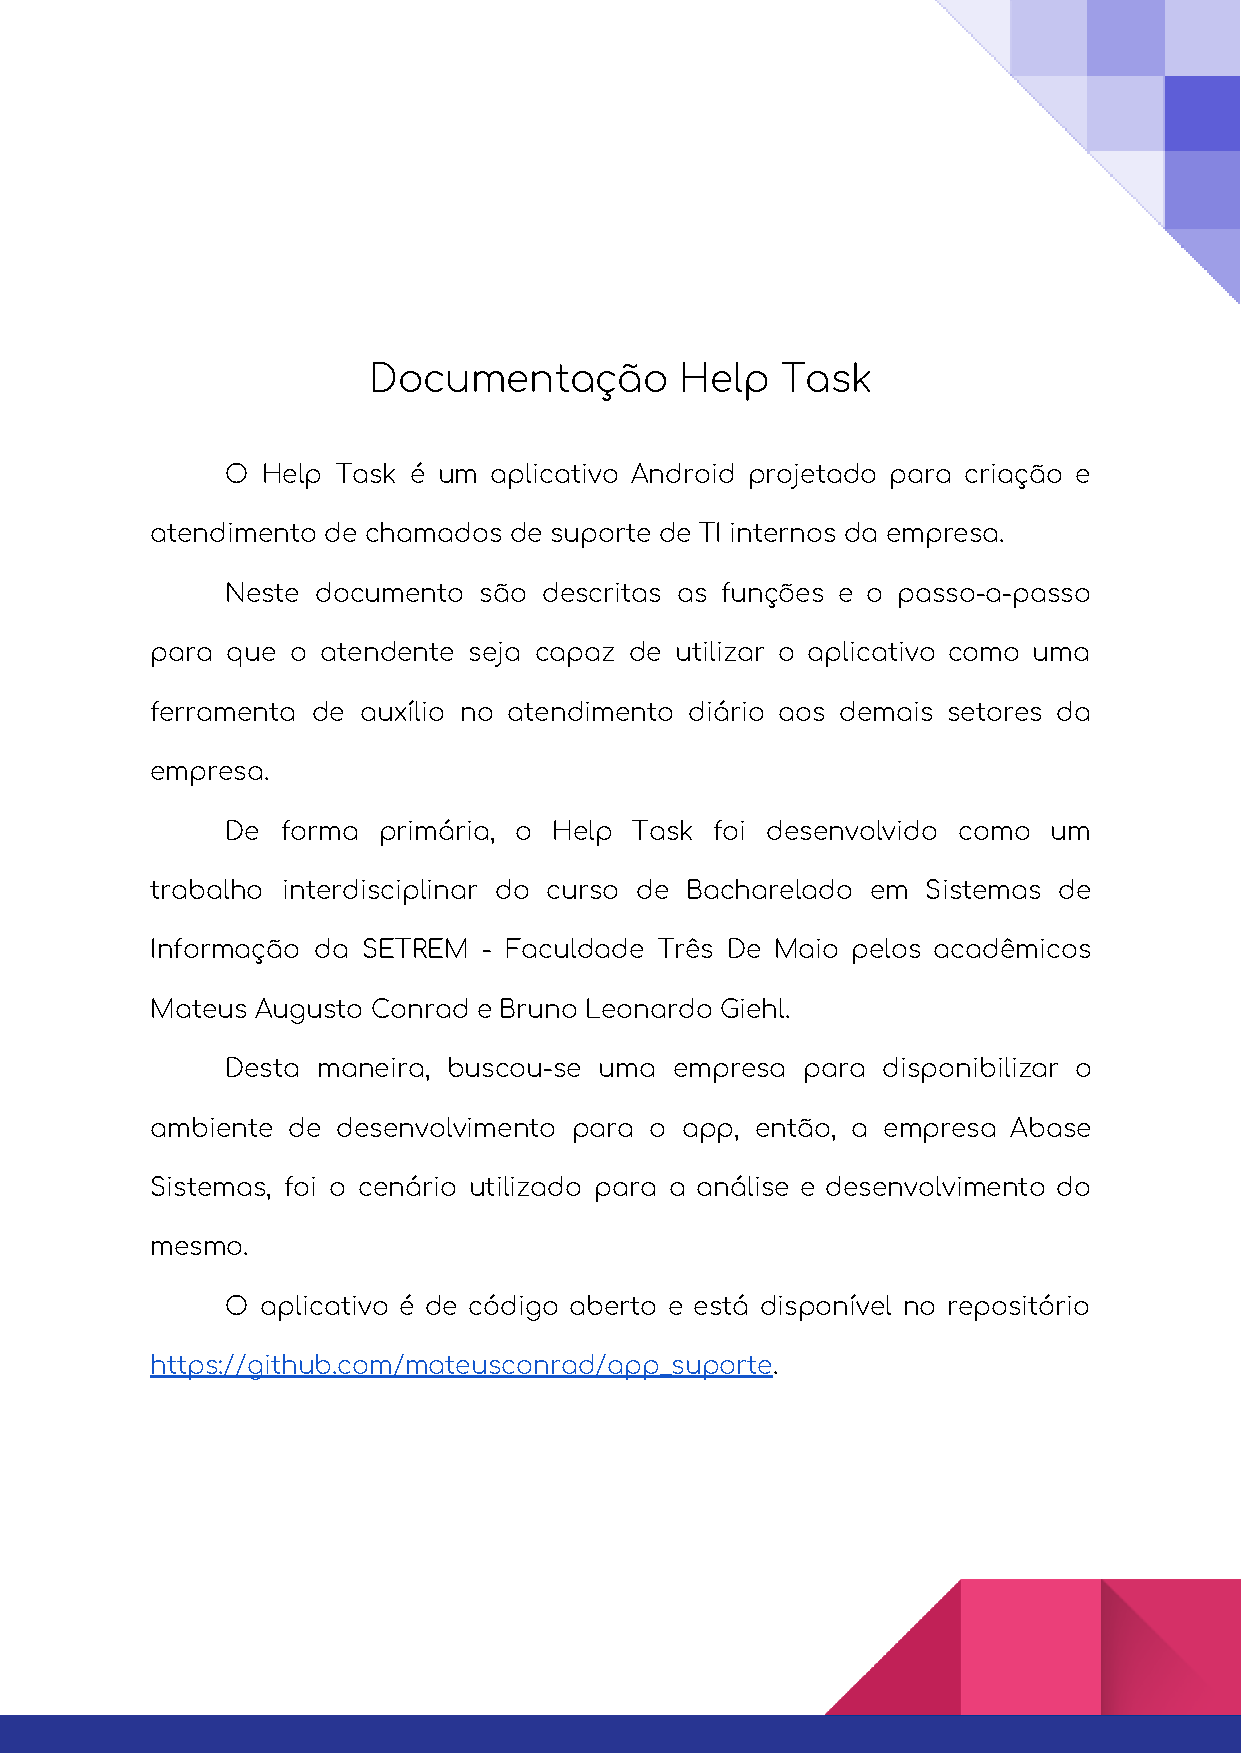
\includepdf[page={-}]{documentacao}

\renewcommand{\thechapter}{APÊNDICE IV -}
\chapter{Resumo Expandido}

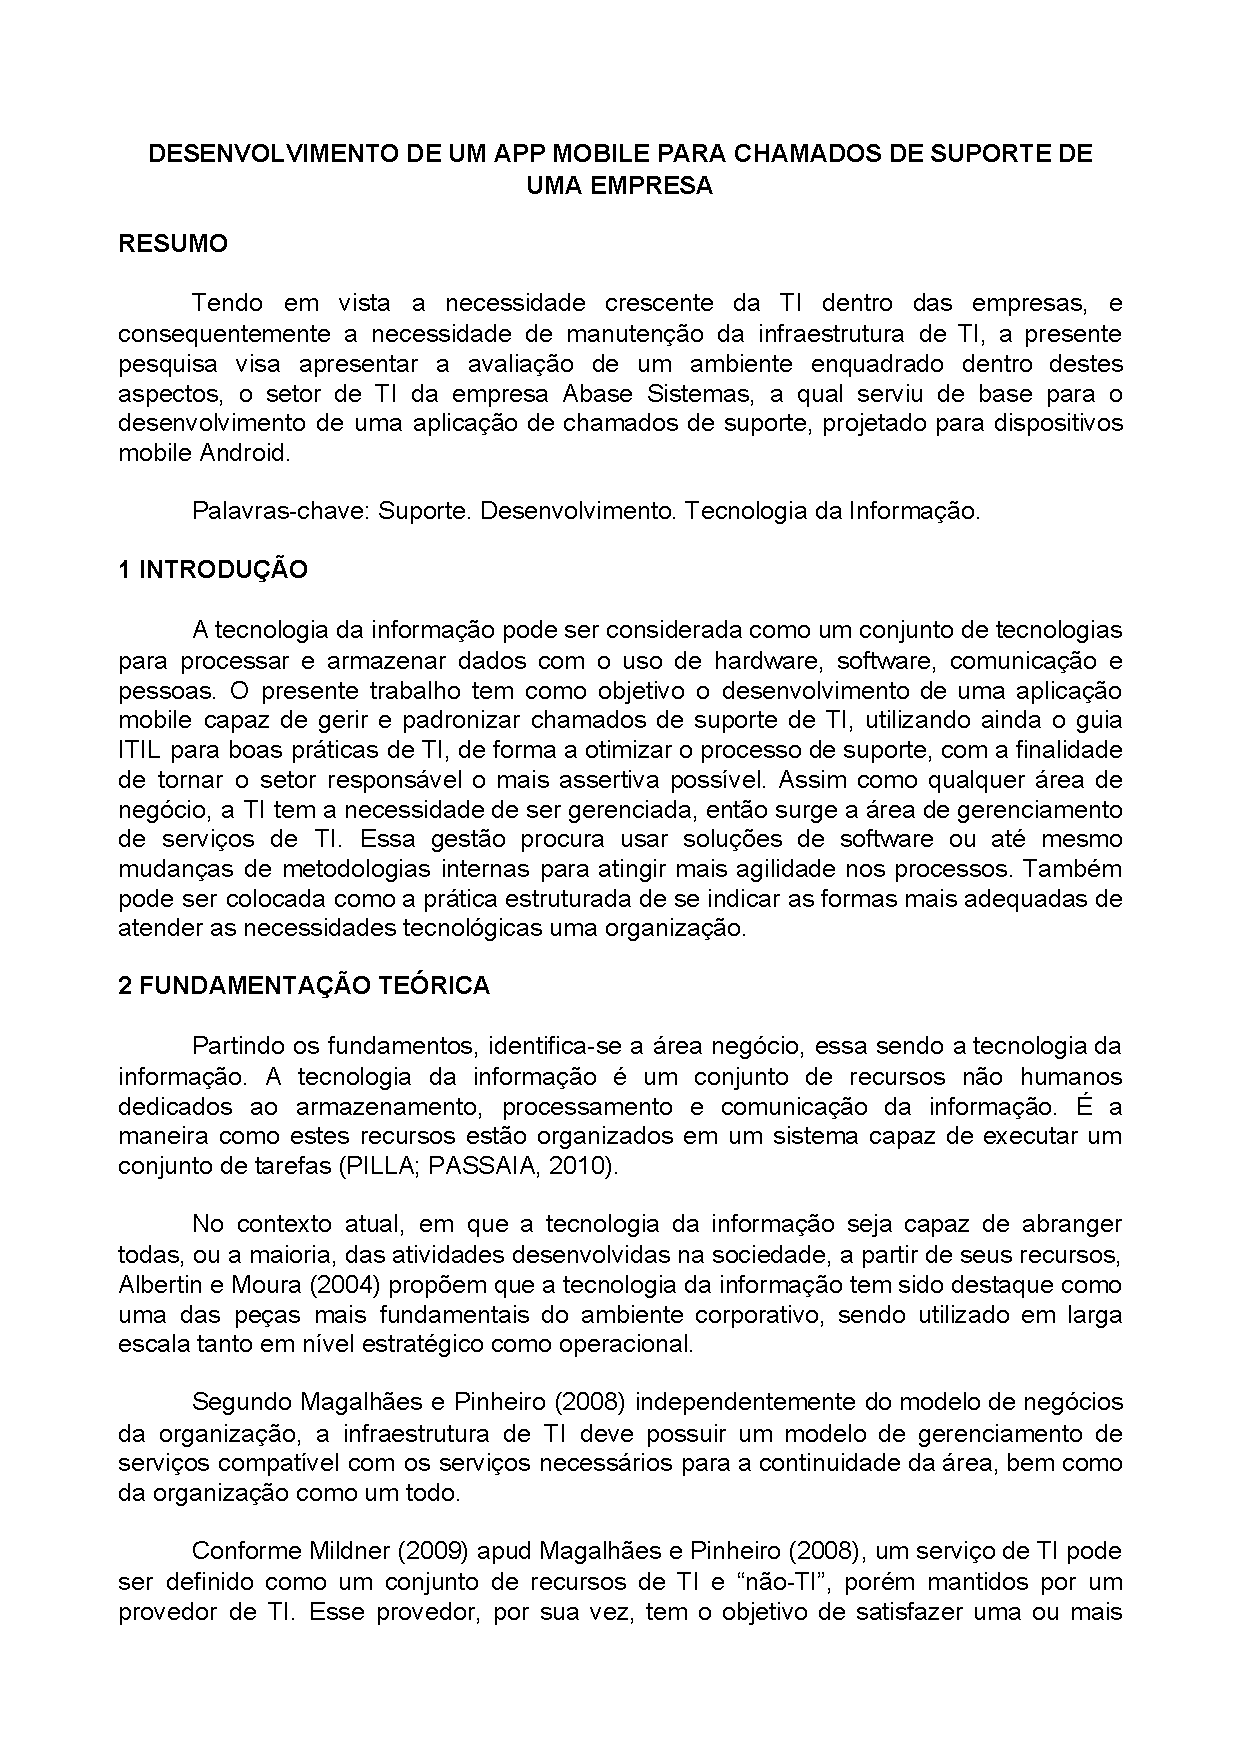
\includepdf[page={-}]{expandido}